\section{SQL}
\subsection*{Teamer}
\begin{frame}{Temaer}
\begin{itemize}
    \item Select
    \item Aggregation
    \item Joins
    \item Update
    \item Insert
    \item Delete
    \item Create and Drop Tables
    \item Datatyper
    \item Constraints
    \item Alt mulig
    \item SQL injections
\end{itemize}
\end{frame}

\subsection*{Enkle Select statements}
\begin{frame}[fragile]{Select}
\begin{minted}{sql}
SELECT director, COUNT(*) as c -- Spalter
FROM movie                     -- Tabeller
WHERE country = "Dabendorf"    -- Betingelser
GROUP BY director              -- Gruppering etter spalter
HAVING c > 3                   -- Betingelser etter gruppering
ORDER BY c DESC                -- Sortering etter spalter 
LIMIT 3;                       -- Velg de første n output linjene
\end{minted}
\end{frame}

\subsection*{Aggregasjonsfunksjoner}
\begin{frame}[fragile]{Aggregation}
\begin{itemize}[<+->]
    \item Count: Teller antall elementer
    \item Sum: Summerer verdier
    \item Avg: Gjennomsnitt av verdier (tilsvarer count/sum)
    \item Min: Minimum
    \item Max: Maksimum
    \item Alle aggregasjonsfunksjoner ignorerer NULL verdier
\end{itemize}
\end{frame}

\subsection*{Joins}
\begin{frame}[fragile]{Join (2 varianter)}
\begin{minted}{sql}
SELECT *                -- Variante 1
FROM film, screening    -- Velg alle tabeller og bruk WHERE
WHERE film.film_id = screening.film_id;
\end{minted}
\pause
\begin{minted}{sql}
SELECT *                -- Variante 2
FROM film               -- Velg en tabell og bruk JOIN og ON
JOIN screening ON film.film_id = screening.film_id;
\end{minted}
\end{frame}

\begin{frame}{Types of Joins}
\begin{itemize}[<+->]
    \item INNER JOIN: Alle rad som finnes i begge tabeller
    \item LEFT (OUTER) JOIN: Alle rad som finnes i begge tabeller og alt fra venstre tabellen
    \item RIGHT (OUTER) JOIN: Alle rad som finnes i begge tabeller og alt fra høyre tabellen
    \item FULL (OUTER) JOIN: Alt fra begge tabeller
    \item \textit{Alt} mener tilsvarende JOIN columns
    \item Ikke-eksisterende verdier fylles med NULL verdier
    \item \dots SELF JOIN, CROSS JOIN, NATURAL JOIN, \dots
\end{itemize}
\end{frame}

\begin{frame}{Venn Diagram}
    \begin{figure}
        \centering
        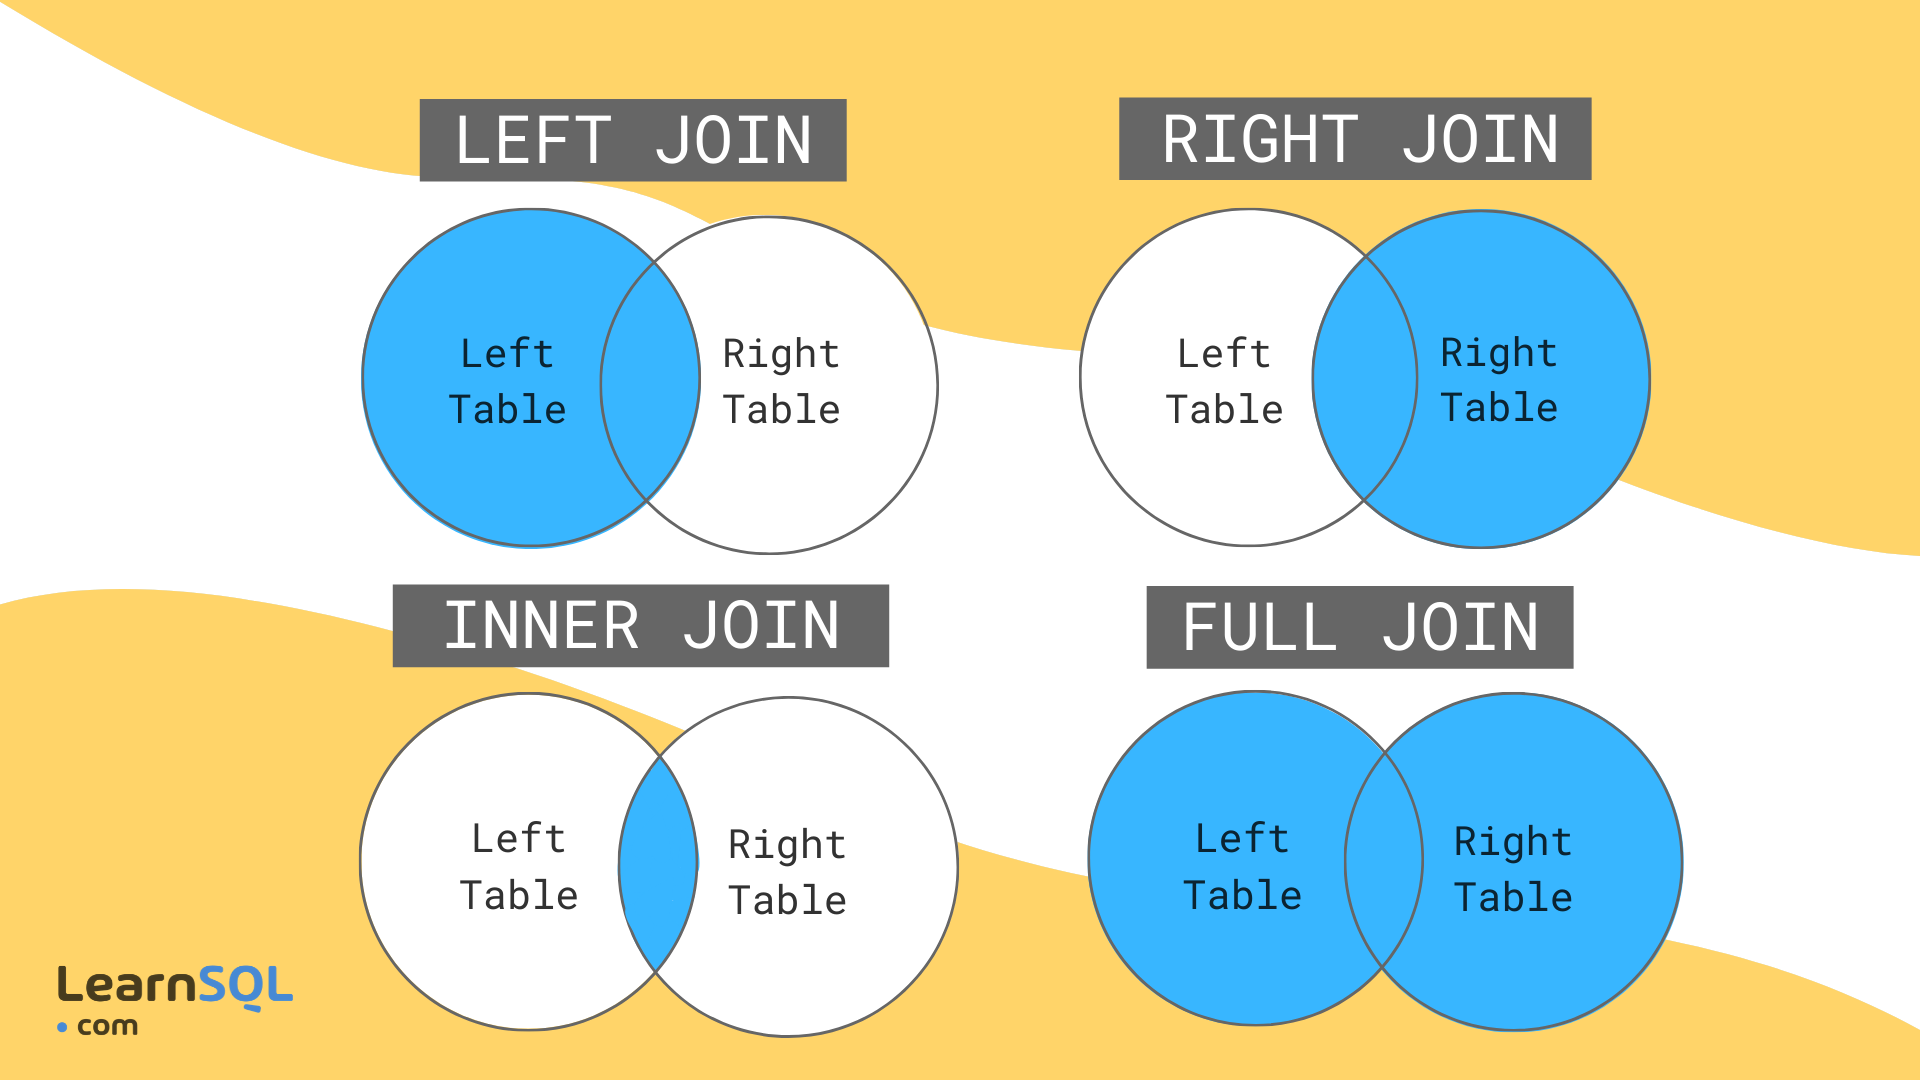
\includegraphics[height = 4.9cm]{images/joins.png}
        \caption{Kilde:
        https://learnsql.com/blog/learn-and-practice-sql-joins/}
        \label{fig:venndiagram}
    \end{figure}
\end{frame}

\begin{frame}%{Eksempel INNER JOIN}
\begin{columns}
    \begin{column}{0.48\textwidth}
        \begin{table}
        \resizebox{2.8cm}{!}{%
        \begin{tabular}{c|c|>{\columncolor[gray]{0.8}}c}
        RuteID & Fra & Til \\\hline
        0 & 2 & 1\\
        1 & 5 & 1\\
        2 & 1 & 2\\
        3 & 3 & 2\\
        4 & 2 & 3\\
        5 & 1 & 4\\
        6 & 1 & 6\\
        7 & 2 & 7
        \end{tabular}
        }
        \end{table}
		
		\vspace{0.2cm}
		
		\begin{table}
		\resizebox{3.5cm}{!}{%
		\begin{tabular}{>{\columncolor[gray]{0.8}}c|l}
		 FlyplassID & By\\\hline
		1 & Bergen\\
		2 & Dabendorf\\
		3 & PorsgruNN\\
		4 & Reykjavík\\
		5 & Oslo
		\end{tabular}
		}
		\end{table}
        
		
 	\end{column}
 	\pause
    \begin{column}{0.48\textwidth}
        \begin{table}
		\resizebox{6cm}{!}{%
		\begin{tabular}{c|c|>{\columncolor[gray]{0.8}}c|>{\columncolor[gray]{0.8}}c|l}
		 RuteID & Fra & Til & FlyplassID & By\\\hline
		 0 & 2 & 1 & 1 & Bergen\\
		 1 & 5 & 1 & 1 & Bergen\\
		 2 & 1 & 2 & 2 & Dabendorf\\
		 3 & 3 & 2 & 2 & Dabendorf\\
		 4 & 2 & 3 & 3 & PorsgruNN\\
		 5 & 1 & 4 & 4 & Reykjavík\\
		\end{tabular}
		}
		\caption{Eksempel: INNER JOIN}
		\end{table}
 	\end{column}
\end{columns}

\end{frame}

\begin{frame}%{Eksempel LEFT JOIN}
\begin{columns}
    \begin{column}{0.48\textwidth}
        \begin{table}
        \resizebox{2.8cm}{!}{%
        \begin{tabular}{c|c|>{\columncolor[gray]{0.8}}c}
        RuteID & Fra & Til \\\hline
        0 & 2 & 1\\
        1 & 5 & 1\\
        2 & 1 & 2\\
        3 & 3 & 2\\
        4 & 2 & 3\\
        5 & 1 & 4\\
        6 & 1 & 6\\
        7 & 2 & 7
        \end{tabular}
        }
        \end{table}
		
		\vspace{0.2cm}
		
		\begin{table}
		\resizebox{3.5cm}{!}{%
		\begin{tabular}{>{\columncolor[gray]{0.8}}c|l}
		 FlyplassID & By\\\hline
		1 & Bergen\\
		2 & Dabendorf\\
		3 & PorsgruNN\\
		4 & Reykjavík\\
		5 & Oslo
		\end{tabular}
		}
		\end{table}
        
		
 	\end{column}
 	\pause
    \begin{column}{0.48\textwidth}
        \begin{table}
		\resizebox{6cm}{!}{%
		\begin{tabular}{c|c|>{\columncolor[gray]{0.8}}c|>{\columncolor[gray]{0.8}}c|l}
		 RuteID & Fra & Til & FlyplassID & By\\\hline
		 0 & 2 & 1 & 1 & Bergen\\
		 1 & 5 & 1 & 1 & Bergen\\
		 2 & 1 & 2 & 2 & Dabendorf\\
		 3 & 3 & 2 & 2 & Dabendorf\\
		 4 & 2 & 3 & 3 & PorsgruNN\\
		 5 & 1 & 4 & 4 & Reykjavík\\
		 6 & 1 & 6 & NULL & NULL\\
         7 & 2 & 7 & NULL & NULL
		\end{tabular}
		}
		\caption{Eksempel: LEFT JOIN}
		\end{table}
 	\end{column}
\end{columns}
    
\end{frame}

\begin{frame}%{Eksempel RIGHT JOIN}
\begin{columns}
    \begin{column}{0.48\textwidth}
        \begin{table}
        \resizebox{2.8cm}{!}{%
        \begin{tabular}{c|c|>{\columncolor[gray]{0.8}}c}
        RuteID & Fra & Til \\\hline
        0 & 2 & 1\\
        1 & 5 & 1\\
        2 & 1 & 2\\
        3 & 3 & 2\\
        4 & 2 & 3\\
        5 & 1 & 4\\
        6 & 1 & 6\\
        7 & 2 & 7
        \end{tabular}
        }
        \end{table}
		
		\vspace{0.2cm}
		
		\begin{table}
		\resizebox{3.5cm}{!}{%
		\begin{tabular}{>{\columncolor[gray]{0.8}}c|l}
		 FlyplassID & By\\\hline
		1 & Bergen\\
		2 & Dabendorf\\
		3 & PorsgruNN\\
		4 & Reykjavík\\
		5 & Oslo
		\end{tabular}
		}
		\end{table}
        
		
 	\end{column}
 	\pause
    \begin{column}{0.48\textwidth}
        \begin{table}
		\resizebox{6cm}{!}{%
		\begin{tabular}{c|c|>{\columncolor[gray]{0.8}}c|>{\columncolor[gray]{0.8}}c|l}
		 RuteID & Fra & Til & FlyplassID & By\\\hline
		 0 & 2 & 1 & 1 & Bergen\\
		 1 & 5 & 1 & 1 & Bergen\\
		 2 & 1 & 2 & 2 & Dabendorf\\
		 3 & 3 & 2 & 2 & Dabendorf\\
		 4 & 2 & 3 & 3 & PorsgruNN\\
		 5 & 1 & 4 & 4 & Reykjavík\\
		 NULL & NULL & NULL & 5 & Oslo
		\end{tabular}
		}
		\caption{Eksempel: RIGHT JOIN}
		\end{table}
 	\end{column}
\end{columns}
    
\end{frame}

\begin{frame}%{Eksempel FULL OUTER JOIN}
\begin{columns}
    \begin{column}{0.48\textwidth}
        \begin{table}
        \resizebox{2.8cm}{!}{%
        \begin{tabular}{c|c|>{\columncolor[gray]{0.8}}c}
        RuteID & Fra & Til \\\hline
        0 & 2 & 1\\
        1 & 5 & 1\\
        2 & 1 & 2\\
        3 & 3 & 2\\
        4 & 2 & 3\\
        5 & 1 & 4\\
        6 & 1 & 6\\
        7 & 2 & 7
        \end{tabular}
        }
        \end{table}
		
		\vspace{0.2cm}
		
		\begin{table}
		\resizebox{3.5cm}{!}{%
		\begin{tabular}{>{\columncolor[gray]{0.8}}c|l}
		 FlyplassID & By\\\hline
		1 & Bergen\\
		2 & Dabendorf\\
		3 & PorsgruNN\\
		4 & Reykjavík\\
		5 & Oslo
		\end{tabular}
		}
		\end{table}
        
		
 	\end{column}
 	\pause
    \begin{column}{0.48\textwidth}
        \begin{table}
		\resizebox{6cm}{!}{%
		\begin{tabular}{c|c|>{\columncolor[gray]{0.8}}c|>{\columncolor[gray]{0.8}}c|l}
		 RuteID & Fra & Til & FlyplassID & By\\\hline
		 0 & 2 & 1 & 1 & Bergen\\
		 1 & 5 & 1 & 1 & Bergen\\
		 2 & 1 & 2 & 2 & Dabendorf\\
		 3 & 3 & 2 & 2 & Dabendorf\\
		 4 & 2 & 3 & 3 & PorsgruNN\\
		 5 & 1 & 4 & 4 & Reykjavík\\
		 6 & 1 & 6 & NULL & NULL\\
         7 & 2 & 7 & NULL & NULL\\
		 NULL & NULL & NULL & 5 & Oslo
		\end{tabular}
		}
		\caption{Eksempel: FULL OUTER JOIN}
		\end{table}
 	\end{column}
\end{columns}
    
\end{frame}


\subsection*{Oppdatere informasjoner}
\begin{frame}[fragile]{Update}
\begin{minted}{sql}
UPDATE book                 -- tabell
SET title = "Der satanarchäolügenialkohöllische Wunschpunsch"
WHERE book_id = 37;         -- betingelse
\end{minted}
\pause
\vspace{-5mm}
\begin{minted}{sql}
UPDATE music                -- tabell
SET title = "Supercalifragilisticexpialidocious",
   artist = "Mary Poppins"  -- oppdatert informasjon
WHERE song_id = 42;         -- betingelse
\end{minted}
\end{frame}

\subsection*{Legg til informasjoner}
\begin{frame}[fragile]{Insert (2 varianter)}
\begin{minted}{sql}
INSERT INTO film (film_id, title, director, genre)
VALUES (7, "Fantômas", "André Hunebelle", "Fransk tull"); 
\end{minted}
\pause
\begin{minted}{sql}
INSERT INTO film    -- spaltenavn ikke nødvendig hvis alle blir brukt
VALUES (7, "Fantômas", "André Hunebelle", "Fransk tull"); 
\end{minted}
\end{frame}

\subsection*{Fjerne informasjoner}
\begin{frame}[fragile]{Delete}
\begin{minted}{sql}
DELETE FROM film        -- tabell
WHERE country = "USA";  -- betingelse
\end{minted}
\end{frame}

\subsection*{Lage nye tabeller}
\begin{frame}[fragile]{Create Table}
\begin{minted}{sql}
CREATE TABLE Persons (
    Person_id int,              -- column name, datatype
    LastName varchar(40) NOT NULL,
    FirstName varchar(40),
    Age int,
    Department_id int UNIQUE,
    PRIMARY KEY (Person_id),    -- primær- og fremmednøkler
    FOREIGN KEY (Department_id) REFERENCES Department(Department_id),
    CHECK (Age>=18)             -- constraints
);
\end{minted}
\end{frame}

\subsection*{Slette tabeller}
\begin{frame}[fragile]{Drop Table}
\begin{minted}{sql}
DROP TABLE eksamenskarakterer;  -- tabell som skal slettes 
\end{minted}
\end{frame}

\subsection*{Datatyper}
\begin{frame}[fragile]{Datatyper}
\begin{minted}{sql}
char(20)            -- 20 tegn med fast lengde
varchar(20)         -- opptil 20 tegn
text                -- tekst med opptil 2^16 tegn
int                 -- integer (tinyint, smallint, bigint)
float(2)            -- float med 2 sifre bak komma
decimal(5,2)        -- 3 sifre før og 2 etter komma
enum ("INF102", "INF234", "INF237") -- en av n verdier
date                -- dato
timestamp           -- unix timestamp
\end{minted}
\end{frame}

\subsection*{Constraints}
\begin{frame}[fragile]{Constraints}
\begin{minted}{sql}
NOT NULL                    -- verdien er ikke NULL
UNIQUE                      -- spalten har ingen verdi flere ganger
PRIMARY KEY(key)            -- NOT NULL + UNIQUE
FOREIGN KEY(key) REFERENCES tabell(key) -- fremmednøkkel
AGE int CHECK (AGE >= 18)   -- betingelse
AGE int DEFAULT 18          -- standardverdi
\end{minted}
\end{frame}

\subsection*{Andre ting}
\begin{frame}[fragile]{Alt mulig}
\begin{minted}{sql}
SELECT DISTINCT                     -- fjerner duplikater
WHERE navn LIKE "A%"                -- alt som starter med A
-- % 0, 1 eller flere tegn
-- _ eksakt et tegn
WHERE category IN ("cake", "bread") -- verdien er i en liste
WHERE age BETWEEN 18 and 65         -- verdien er i en range
WHERE EXISTS (SELECT ...)           -- verdien finnes i en annen query
(SELECT ...) UNION (SELECT ...)     -- union av to queries
\end{minted}
\end{frame}

\begin{frame}[fragile]{Alt mulig}
\begin{minted}{sql}
SELECT Order_id, Price,
CASE    -- if betingelser i SELECT
    WHEN Price > 30 THEN "Won't pay freight"
    ELSE "Freight costs 10\$"
END AS FrightCost
FROM OrderDetails; 
\end{minted}
\end{frame}

\subsection*{Spørretid}
\begin{frame}{Spørsmål?}
    \begin{figure}
        \centering
        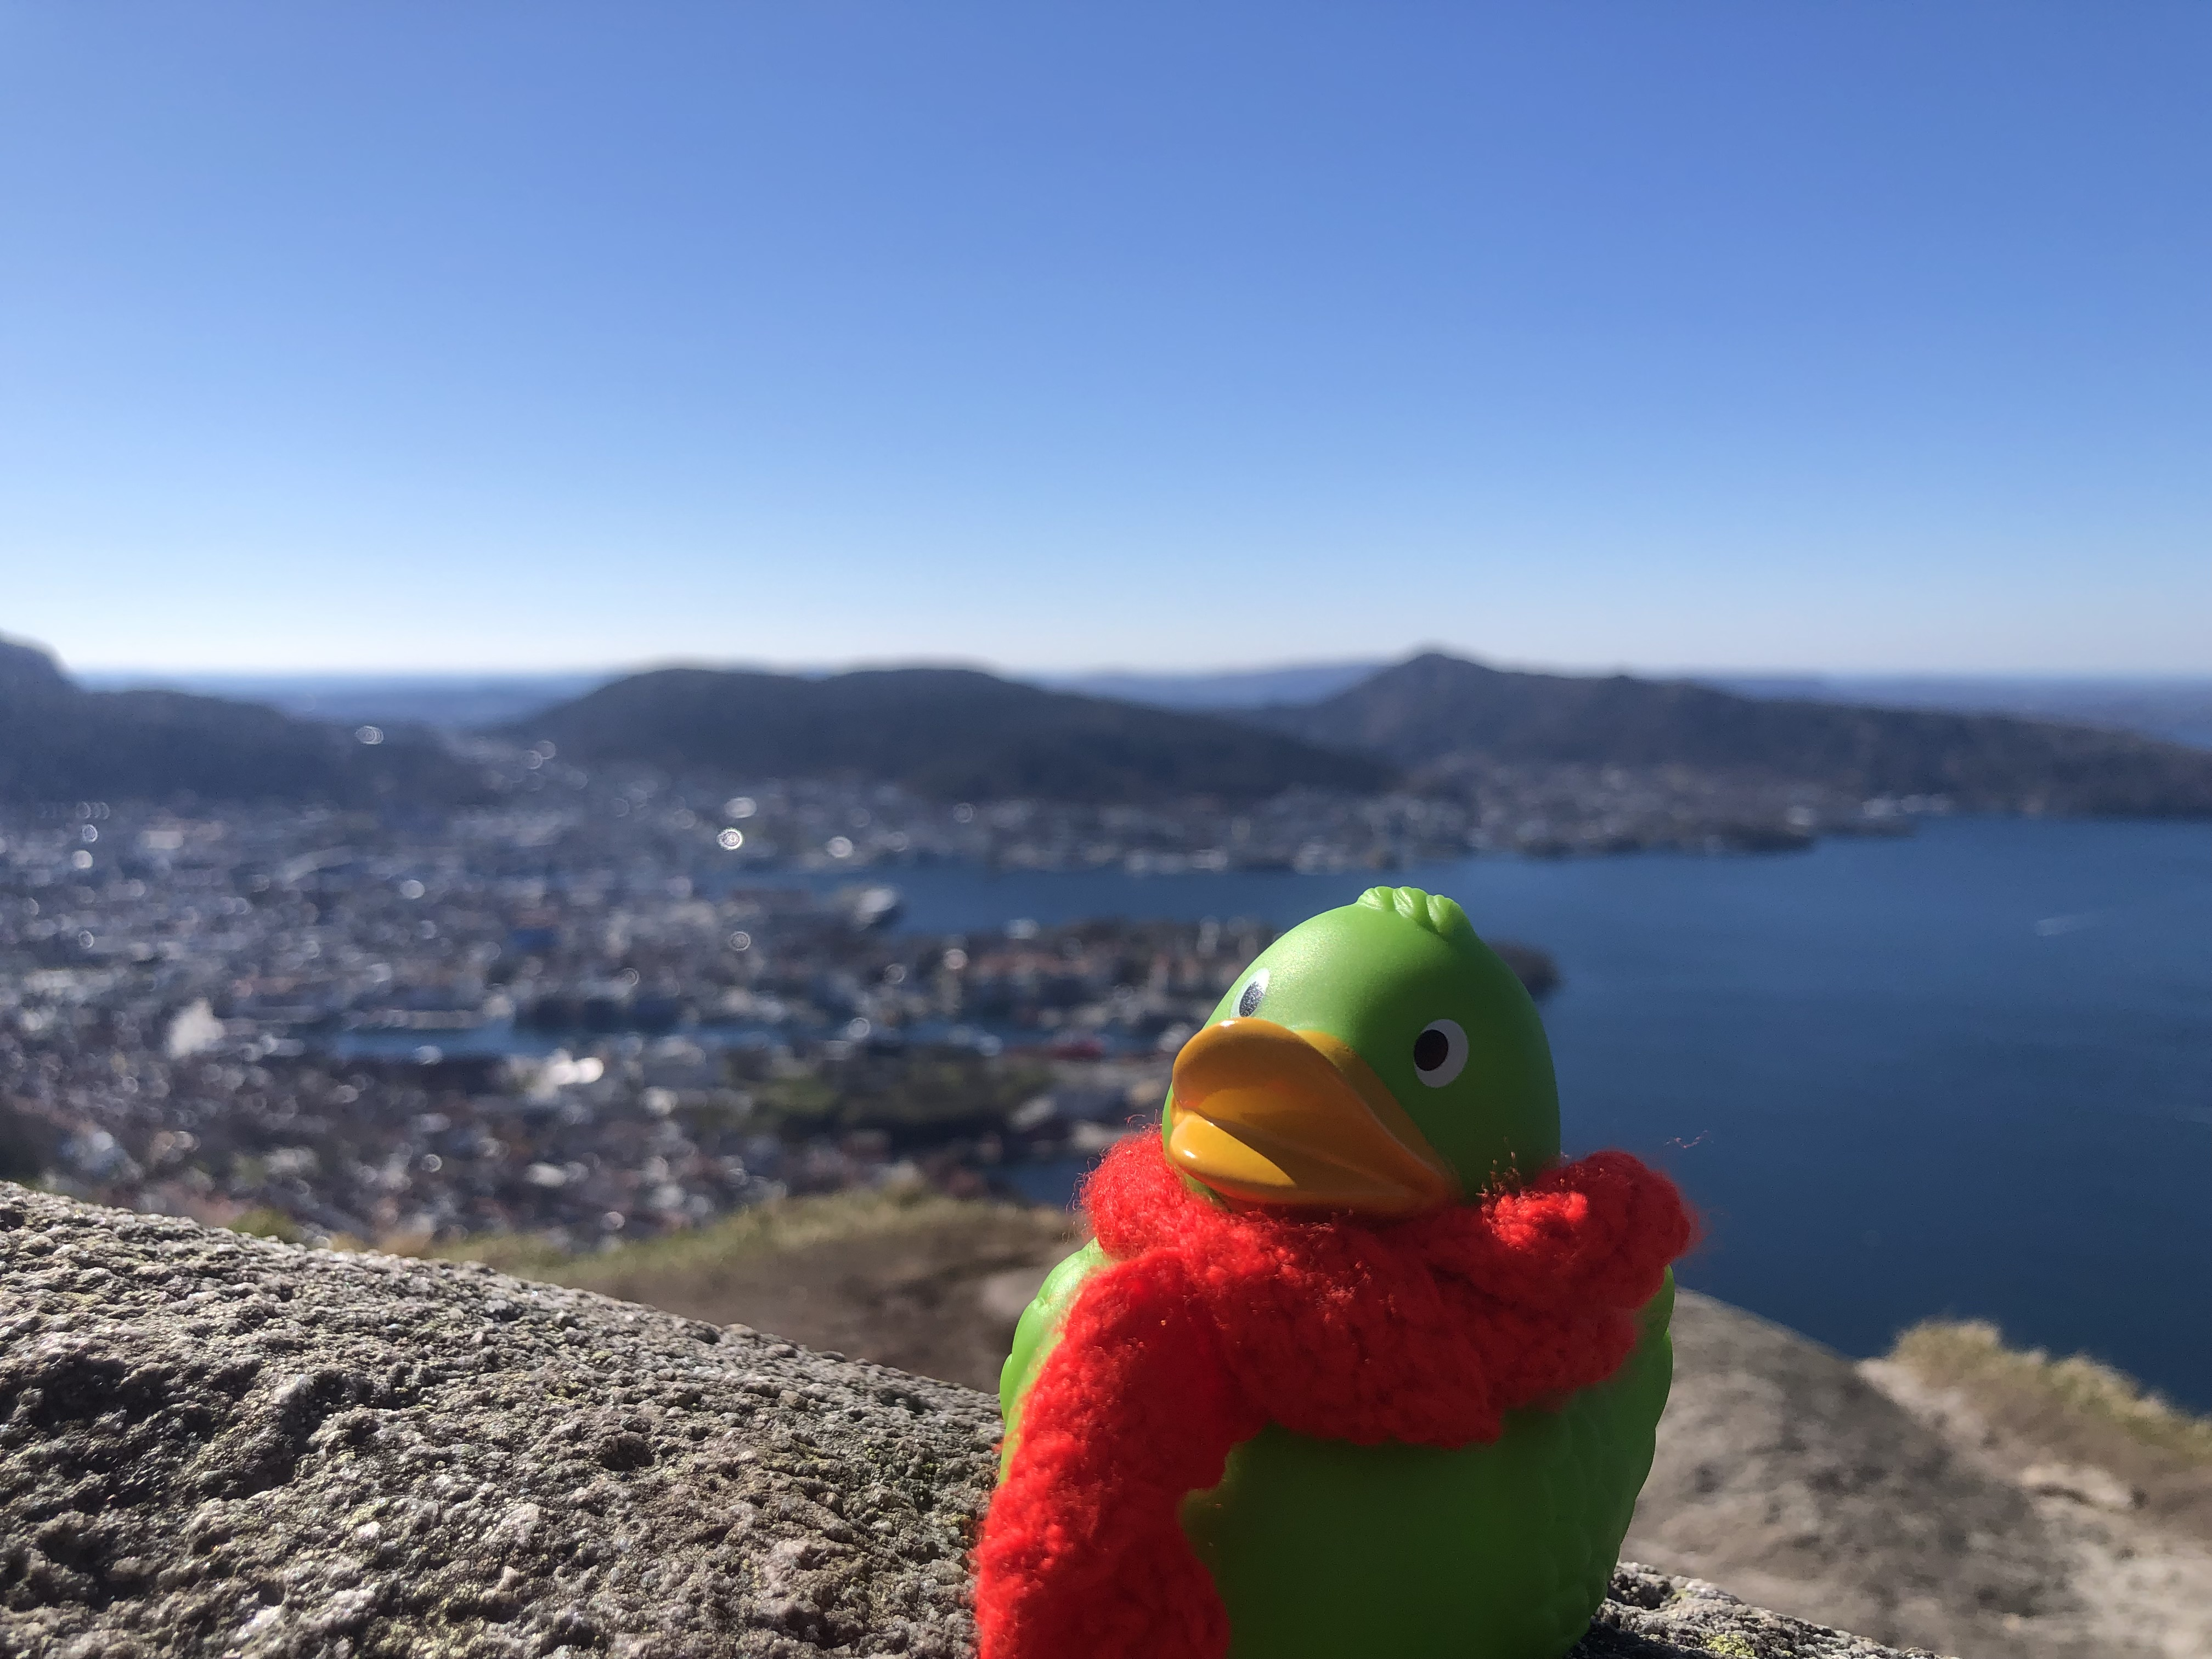
\includegraphics[height = 4.9cm]{images/guillaume1.jpg}
        \caption{Guillaume på Sandviksfjellet}
        \label{fig:guillaume1}
    \end{figure}
\end{frame}